%%%%%%%%%%%%%%%%%%%%%%%%%%%%%%%%%%%%%%%%%
% University Assignment Title Page 
% LaTeX Template
% Version 1.0 (27/12/12)
%
% This template has been downloaded from:
% http://www.LaTeXTemplates.com
%
% Original author:
% WikiBooks (http://en.wikibooks.org/wiki/LaTeX/Title_Creation)
%
% License:
% CC BY-NC-SA 3.0 (http://creativecommons.org/licenses/by-nc-sa/3.0/)
% 
% Instructions for using this template:
% This title page is capable of being compiled as is. This is not useful for 
% including it in another document. To do this, you have two options: 
%
% 1) Copy/paste everything between \begin{document} and \end{document} 
% starting at \begin{titlepage} and paste this into another LaTeX file where you 
% want your title page.
% OR
% 2) Remove everything outside the \begin{titlepage} and \end{titlepage} and 
% move this file to the same directory as the LaTeX file you wish to add it to. 
% Then add \input{./title_page_1.tex} to your LaTeX file where you want your
% title page.
%
%%%%%%%%%%%%%%%%%%%%%%%%%%%%%%%%%%%%%%%%%
%\title{Title page with logo}
%----------------------------------------------------------------------------------------
%   PACKAGES AND OTHER DOCUMENT CONFIGURATIONS
%----------------------------------------------------------------------------------------

\documentclass[14pt]{extarticle}
% \documentclass[bibliography=totocnumbered]{scrartcl}
% \usepackage[english]{babel}
\usepackage[russian]{babel}
\usepackage[utf8x]{inputenc}
\usepackage{float}
\usepackage{amsmath}
\usepackage{graphicx}
\usepackage{subcaption}
\usepackage[colorinlistoftodos]{todonotes}
\renewcommand{\baselinestretch}{1.5}
\usepackage[left=3cm,right=1cm,top=1.5cm,bottom=2cm]{geometry}
\setlength{\parindent}{0mm}
\setlength{\parskip}{1em}
\usepackage{hyperref}
\hypersetup{
    colorlinks,
    citecolor=black,
    filecolor=black,
    linkcolor=black,
    urlcolor=black
}

\begin{document}
\begin{titlepage}

% \newgeometry{margin=2cm}
\newcommand{\HRule}{\rule{\linewidth}{0.5mm}} % Defines a new command for the horizontal lines, change thickness here

\center % Center everything on the page
 
%----------------------------------------------------------------------------------------
%   HEADING SECTIONS
%----------------------------------------------------------------------------------------
\textsc {
\footnotesize{
минобрнауки россии\\
федеральное государственное бюджетное образовательное учреждение\\
высшего профессионального образования}\\
\large{Воронежский государственный университет}
}\\[1.0cm] % Name of your university/college


\textsc{\largeФакультет компьютерных наук}\\ % Major heading such as course name
\textsc{\footnotesize010200 Математика и компьютерные науки}\\[1.0cm] 
\textsc{\Large курсовая работа}\\[0.5cm] % Minor heading such as course title


%----------------------------------------------------------------------------------------
%   TITLE SECTION
%----------------------------------------------------------------------------------------

\HRule \\[0.4cm]
{ \huge \bfseries Ультразвуковой стетоскоп}\\[0.4cm] % Title of your document
\HRule \\[1.5cm]
 
%----------------------------------------------------------------------------------------
%   AUTHOR SECTION
%----------------------------------------------------------------------------------------


\begin{flushleft} \large
\emph{Зав. кафедрой:} С.Д. \textsc{Кургалин}, д. ф-м н., проф.\\
\emph{Студент:} А.А. \textsc{Родионов}, 3 курс, гр 6.1 \\ % Your name
\emph{Руководитель:} Я.А. \textsc{Туровский}, к. мед. н , доцент % Supervisor's Name
\end{flushleft}


% If you don't want a supervisor, uncomment the two lines below and remove the section above
% \Large \emph{Author:}\\
% John \textsc{Smith}\\[3cm] % Your name

%----------------------------------------------------------------------------------------
%   DATE SECTION
%----------------------------------------------------------------------------------------
\vfill % Fill the rest of the page with whitespace
\begin{center}
Воронеж 2017
\end{center}
\end{titlepage}

\tableofcontents
\newpage 
\section{Введение}
\subsection{Постановка проблемы}
Аускультация (выслушивание) звуков, исходящих от различных органов - одна из областей медицинской диагностики. Прибор для выслушивания звуков называется стетоскоп. Стетоскопы бывают акустические и электронные. Акустический стетоскоп передает звук от пациента непосредственно в ухо врачу. У электронных есть микрофон, который передает звук либо через динамики врачу, либо записывает для дальнейшего анализа.

Проблемой существующих на рынке электронных стетоскопов является невысокое качество звука. Под невысоким качеством звука подразумевается низкая частота дискретизации получаемого на выходе сигнала и как следствие неспособность выдавать данные о высокочастотном диапазоне звука (в частности ультразвука).

Эти стетоскопы теряют массу информации, которая может быть полезна врачам для осуществления медицинской диагностики пациентов.

\subsection{Цель}
Целью данной курсовой работы является создание доступного и простого в производстве цифрового стетоскопа. Стетоскоп должен быть способен регистрировать высокое качество звука. Он должен иметь высокую частоту дискретизации (600 кГц) и способен регистрировать сигнал в ультразвуковом диапозоне (до 100-300кГц)

В данной работе описывается создание ультразвукогого стетоскопа.

В ходе работы был создан рабочий прототип прибора. Прибор позволяет получать сигнал от ультразвукового микрофона. Также было написано програмное обеспечение к этому прибору. Програмное обеспечение позволяет позволяет записывать и анализировать звуковые сигналы в реальном времени. Есть возможность рассмотреть различные характеристики сигнала, такие как спектр Фурье, скользящее среднее. Также есть возможность записывать аудиосигнал на жесткий диск для его последующей обработки.

\subsection{Применение прибора на практике}
Устройство планируется использоваться в медицине: анализ ультразвуковой составляющей звука от сердца и легких.

Данный прибор может использоваться в медицине для получения и анализа сигнала высокого качества. Например звук сердца и лёгких. 

Это устройство поможет лучше анализировать звук сердца. С помошью визуализации сигнала можно получить больше информации о звуке внутренних органов, чем простое прослушивание.

Также прибор можно использовать в других областях, где необходим анализ ультразвука. 

Например изучение дельфинов или летучих мышей. 

Сердечно-сосудистые заболевания - самая распространенная причина смерти в мире по данным Всемирной Организации Здравоохранения (ВОЗ). Также распространенными являются заболевания легких. Своевременное наблюдение за состоянием сердца и легких, и обнаружение заболеваний - важная задача здравоохранения.

\newpage  
\section{Описание аппаратной части разработанной системы}
Разработанная информационная система состоит из следующих частей:
\begin{enumerate}
  \item Врач
  \item Пациент (диагностируемы)
  \item Мембрана и соединительная трубка от аналогового акустического стетоскопа.
  \item Усилитель
  \item Аналого цифровой преобразователь
  \item Компьютер
  \item Удаленный сервер для высокопроизводительных вычислений
\end{enumerate}

Устройство состоит из нескольких частей. С одной стороны к соединительной трубке подсоединяется мембрана, с другой - микрофон. Мембрана и трубка присоединяется к микрофону для подавления шумов и лучшей передачи звука от сердца/легких. Сигнал с микрофона подается на усилитель. С усилителя сигнал подается на Аналогово-Цифровой-Преобразователь (АЦП). Аналогово-Цифровой-Преобразователь подключается к компьютеру через USB-порт.

\begin{center}
Краткая схема устройства:\\
\noindent\small{{Мембрана → Соединительная Трубка → Микрофон → Усилитель → АЦП → Компьютер}}
\end{center}

% \begin{figure}[H]
% \centering
% 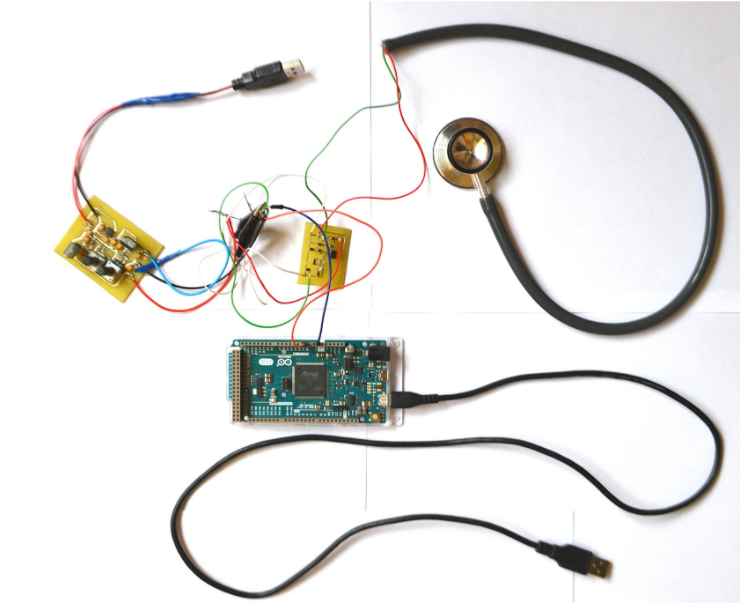
\includegraphics[width=14cm]{hardware.png}
% \caption{Собранный прототип}
% \end{figure}

\subsection{Описание микрофона}
В качестве микрофона был выбран SWEN MK-200. \\

\begin{table}[h]
\centering
\label{my-label}
\begin{tabular}{|l|l|}
\hline
Чувствительность, дБ           & -60 ± 3                    \\ \hline
Диапазон частот, Гц            & 50 – 16 000                \\ \hline
Размер микрофонного модуля, мм & 9×7                        \\ \hline
Тип разъема                    & мини-джек Ø 3,5 мм (3 pin) \\ \hline
Длина кабеля, м                & 1,8                        \\ \hline
Вес, г                         & 63                         \\ \hline
\end{tabular}
\caption{Технические характеристики SWEN MK-200}
\end{table}

Микрофон был вынут из стандартного корпуса, чтобы лучше соединиться с трубкой, ведущей к мембране.

\subsection{Описание усилителя}
Усилитель для микрофона был создан самостоятельно в рамках данной работы.

Была выбрана следующая схема усилителя:

\begin{figure}[H]
\centering
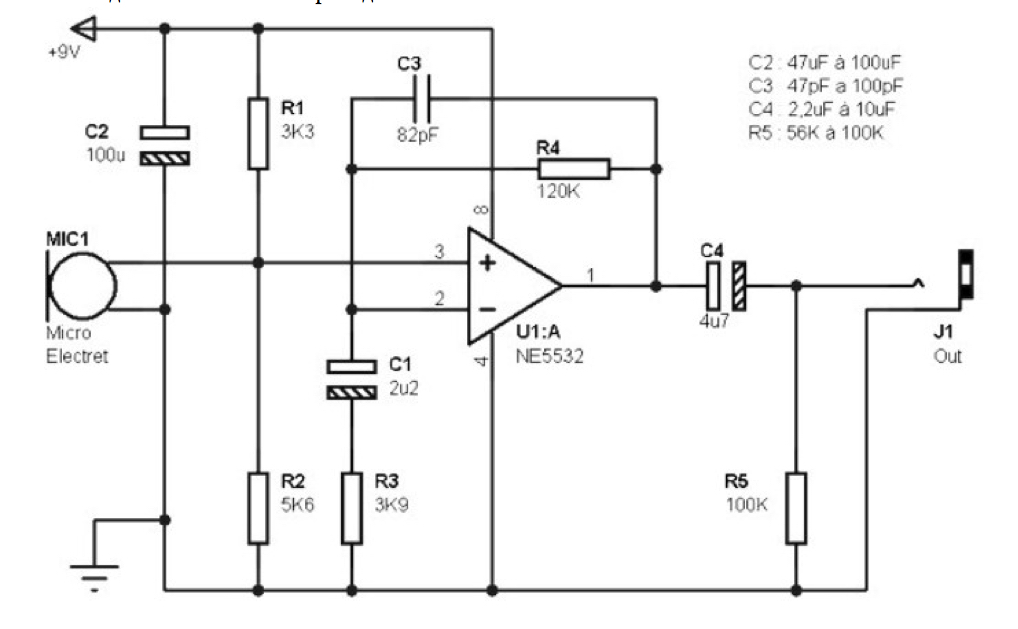
\includegraphics[width=14cm]{circuit.jpg}
\caption{Схема усилителя сигнала}
\end{figure}

В качестве операционного усилителя был выбран \textbf{MCP6022} от производителя Microchip. Это усилитель типа Rail-to-Rail SO-8.

SOIC или просто SO (small-outline-integrated-circuit), а также SOP (Small-Outline Package) корпус микросхем, предназначенный для поверхностного монтажа, занимающий на печатной плате на 30-50\% меньше площади чем аналогичный корпус DIP, а также имеющий на 50-70\% меньшую толщину. Обычно в обозначении также указывается число выводов.

В данный усилитель встроены High-Pass и Low-Pass фильтры. High-Pass фильтрует частоты сигнала меньше 1Гц. Low-Pass фильтрует частоты выше 100кГц. Меняя конденсатор С3, можно менять частоту среза LowPass фильтра. Усиление схемы зависит от резисторов R3 и R4. На текущий момент усиление составляет порядка 100.

Ниже приводятся параметры операционного усилителя.

\begin{table}[h]
\centering
\label{my-label}
\begin{tabular}{|l|l|}
\hline
Полоса частот                  & 10МГц                      \\ \hline
Уровень шума                   & 8.7 нВ/√Гц                 \\ \hline
Количество каналов             & 2                          \\ \hline
Напряжение питания             & 2.5В --- 5.5В              \\ \hline
Напряжение смещения            & $\pm500\mu V $             \\ \hline
Гармонические искажения        & 0.00053\%                  \\ \hline
Температурный диапазон         & -40°C --- +85°C            \\ \hline
Тип корпуса                    & SO-8                       \\ \hline
\end{tabular}
\caption{Технические характеристики операционного усилителя MCP6022}
\end{table}

\begin{figure}[H]
\centering
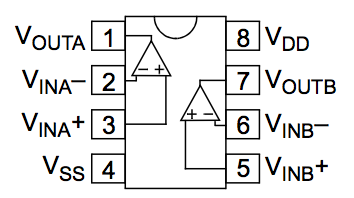
\includegraphics[width=12cm]{op-amp.png}
\caption{Распиновка операционного усилителя}
\end{figure}

\begin{figure}[H]
\begin{subfigure}{0.5\textwidth}
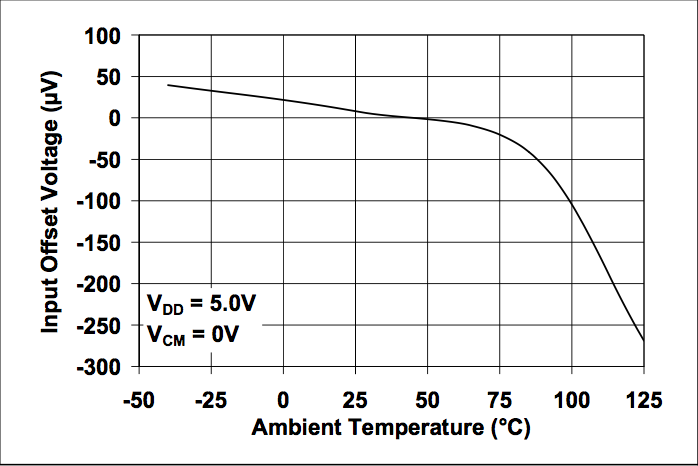
\includegraphics[width=0.9\linewidth, height=5cm]{op-amp-plot1.png} 
\caption{Напряжение смещения --- Температура}
% \label{fig:subim1}
\end{subfigure}
\begin{subfigure}{0.5\textwidth}
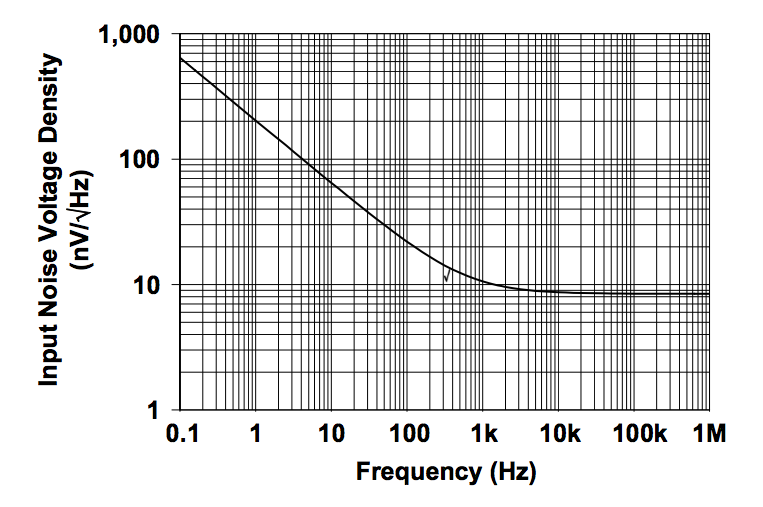
\includegraphics[width=0.9\linewidth, height=5cm]{op-amp-plot2.png}
\caption{Шум --- Частота}
% \label{fig:subim2}
\end{subfigure}

\vspace{10mm} % vertical space
 
\begin{subfigure}{0.5\textwidth}
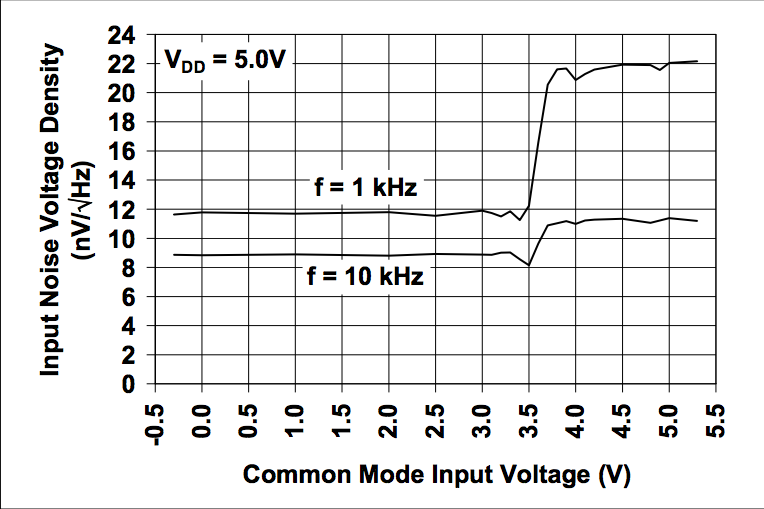
\includegraphics[width=0.9\linewidth, height=5cm]{op-amp-plot3.png} 
\caption{Шум - Напряжение смещения}
% \label{fig:subim1}
\end{subfigure}
\begin{subfigure}{0.5\textwidth}
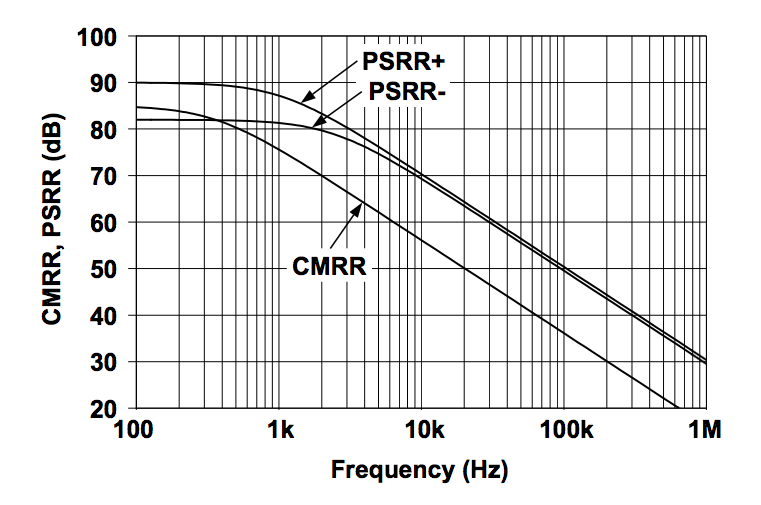
\includegraphics[width=0.9\linewidth, height=5cm]{op-amp-plot4.png}
\caption{CMRR --- Частота}
% \label{fig:subim2}
\end{subfigure}

\vspace{10mm} %vertical space

\begin{subfigure}{0.5\textwidth}
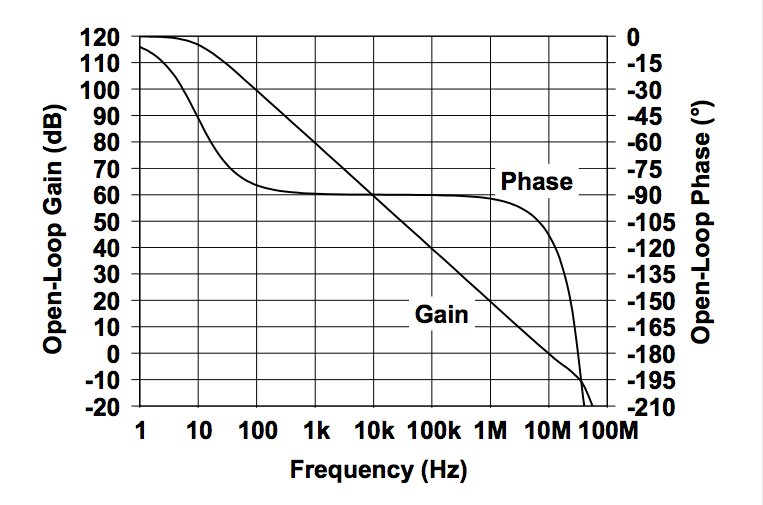
\includegraphics[width=0.9\linewidth, height=5cm]{op-amp-plot5.png} 
\caption{Коэффициент усиления - Частота}
% \label{fig:subim1}
\end{subfigure}
\begin{subfigure}{0.5\textwidth}
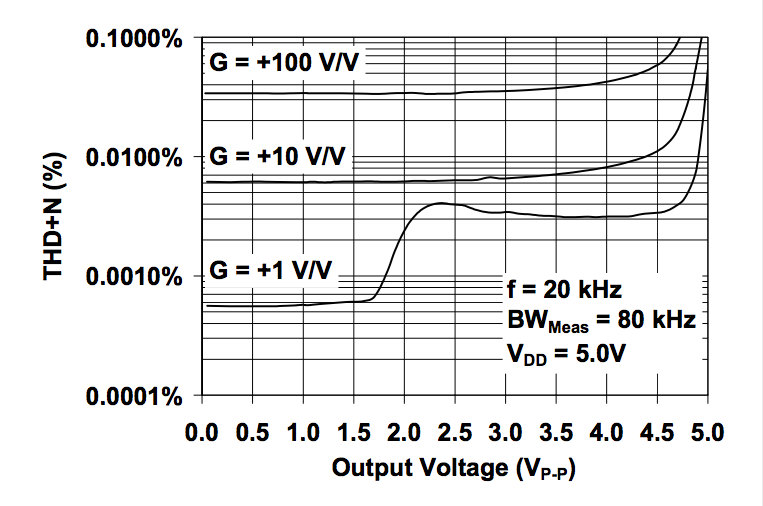
\includegraphics[width=0.9\linewidth, height=5cm]{op-amp-plot6.png}
\caption{\small{Гармонические искажения --- Вых. напряжение (f=20кГц)}}
% \label{fig:subim2}
\end{subfigure}

\caption{Параметры операционного усилителя}
\label{fig:image2}
\end{figure}

Разработка платы усилителя велась в программе Sprint Layout. Ниже представлен скриншот макета платы из этой программы.

\begin{figure}[H]
\centering
% 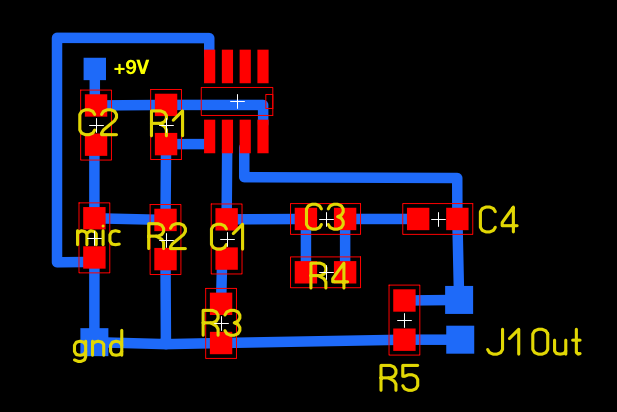
\includegraphics[width=14cm]{sprint-layout-circuit.png}
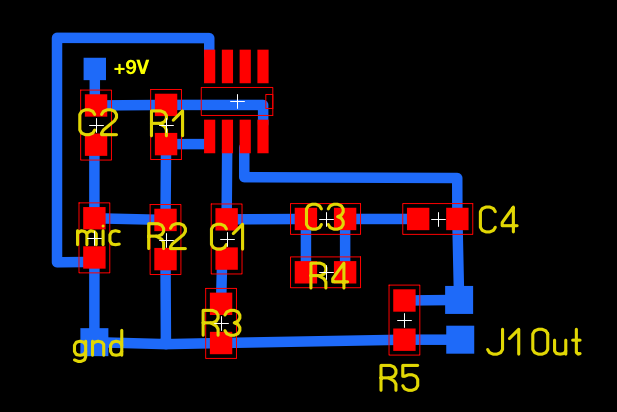
\includegraphics[width=\textwidth]{sprint-layout-circuit.png}
\caption{Схема печатной платы усилителя}
\end{figure}

Печатная плата изготавливалась при помощи печати на лазерном принтере методом травления текстолита. 
\subsection{АЦП}
В качестве аналого цифрового преобразователя был выбран ЛА-н10-12USB от компании ЗАО "Руднев-Шиляев". Также стетоскоп тестировался на АЦП E-140 от компании LCard. 

Предназначение АЦП – преобразование непрерывных (аналоговых) входных сигналов в цифровую форму для дальнейшей обработки с помощью компьютера.

\begin{table}[h]
\centering
\label{my-label}
\begin{tabular}{|l|l|}
                                                                      \hline
Число аналоговых входов            & 2                             \\ \hline
Минимальная частота дискретизации  & 1.25МГц                       \\ \hline
Максимальная частота дискретизации & 80МГц                         \\ \hline
Объем буффера памяти               & $2\times10^{19}=524288$       \\ \hline
Разрядность                        & 12бит (4096 значений)         \\ \hline
Входное сопротивление              & 50Ом                          \\ \hline
Разъем                             & BNC                           \\ \hline
Диапазоны входного напряжения      & $\pm2V;\pm1V;\pm0.4V;\pm0.2V$ \\ \hline
Защита по входному напряжению      & $\pm5V$                       \\ \hline
Дифференциальная нелинейность      & $\pm1.2$ МЗР                  \\ \hline
Интегральная нелинейность          & $\pm1.5$ МЗР                  \\ \hline
Ошибка сдвига                      & $\pm0.15\%$                   \\ \hline
Интерфейс                          & USB                           \\ \hline
Потребляемая мощность              & 12В, 0.7А                     \\ \hline
Масса                              & 400г                          \\ \hline
\end{tabular}
\caption{Технические характеристики АЦП ЛА-н10-12USB}
\end{table}

\textbf{Интегральная нелинейность} - отклонение по вертикальной оси точек реальной характеристики от идеальной характеристики преобразования, делящих пополам расстояние по оси абцисс между средними значениями пороговых уровней характеристики преобразования. Измеряется в процентах или  МЗР.

\textbf{Дифференциальная нелинейность} - отклонение разности двух аналоговых сигналов от значения, соответствующего единице МЗР.

Данный АЦП работает в режиме старт-стоп. Другими словами он периодически производит запуск, сбор данных(в буффер) и остановку. Это один полный цикл сбора данных. При этом полезное время - это сбор данных, а старт и стоп - бесполезное.

Время, за которое АЦП совершает полный цикл сбора данных и соотношение полезного и бесполезного времени отличается в зависимости от частоты дискретизации и размера буффера. Были произведены замеры времени для различных значений частоты дискретизации и размера буффера и были составлены следующие таблицы.

Во всех таблицах X: размер буффера, Y: частота дискр.

\begin{figure}[H]
\centering
% 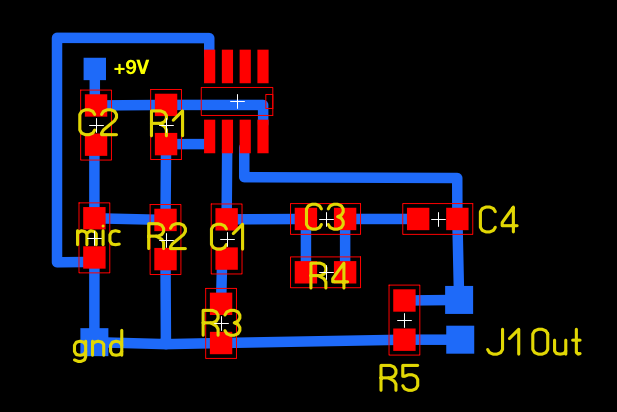
\includegraphics[width=14cm]{sprint-layout-circuit.png}
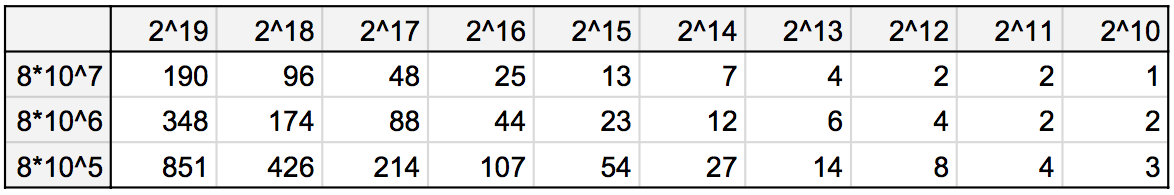
\includegraphics[width=\textwidth]{cycle-time.png}
\caption{Время на полный цикл (мс)}
\end{figure}

\begin{figure}[H]
\centering
% 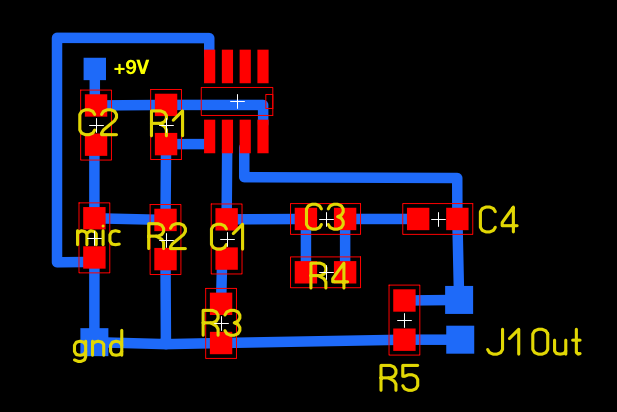
\includegraphics[width=14cm]{sprint-layout-circuit.png}
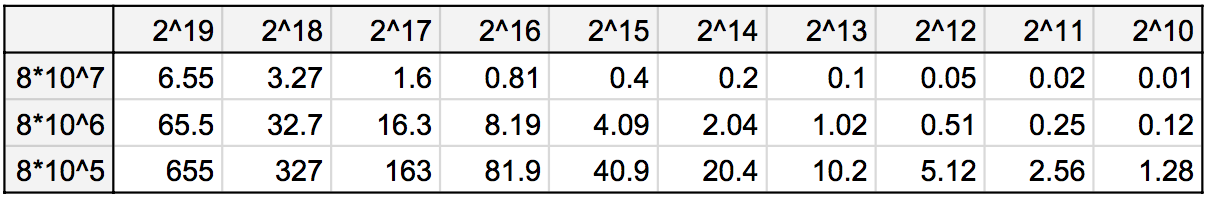
\includegraphics[width=\textwidth]{good-time.png}
\caption{Полезное время (мс)}
\end{figure}

\begin{figure}[H]
\centering
% 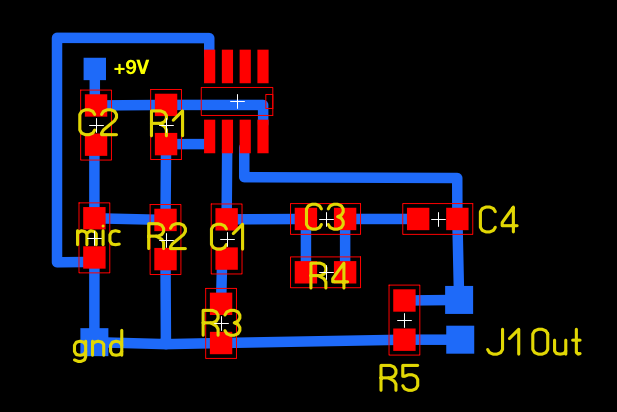
\includegraphics[width=14cm]{sprint-layout-circuit.png}
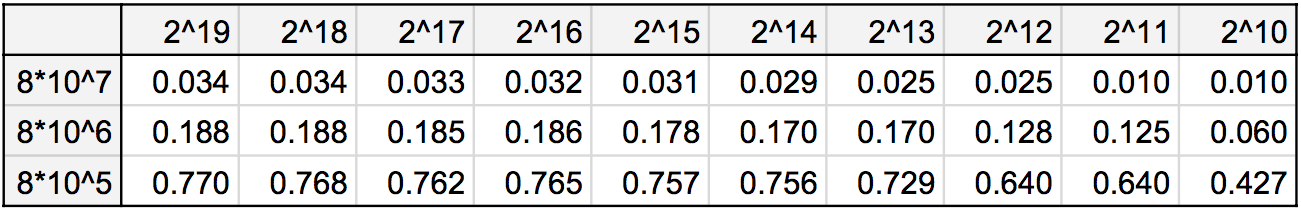
\includegraphics[width=\textwidth]{bad-div-by-good.png}
\caption{Отношение полезного времени к полному}
\end{figure}

\newpage
\section{Описание программного обеспечения}
В рамках данной работы было написано програмное обеспечение для работы с ультразвуковым стетоскопом. Програмное обеспечение написано на языке C\# для платформы Windows.

В функционал програмного обеспечения входит:
\begin{itemize}
  \item Получение сигнала от АЦП ЛА-н10-12USB
  \item Отображение сигнала в реальном времени на экране в виде графика
  \item Отображение спектра сигнала полученного в результате быстрого преобразования Фурье
  \item Отображение скользящего среднего сигнала
  \item Возможность записи сигнала на жесткий диск для последующей обработки
\end{itemize}

\subsection{Инструкция по установке ПО}
\begin{itemize}
  \item Скачать драйверы для АЦП ЛА-н10-12USB по ссылке:\\ \url{http://rudshel.ru/software.html}
  \item Запустить и установить файл \verb|RShUSBDriver_XP_Vista_7_8_x86_x64_SDK2_2.0.x.y.exe| (драйверы для USB устройств)
  \item Запустить и установить файл \verb|RshSDKSetup_2.0.x.y.exe| (средства разработки ПО (SDK))
  \item Скачать проект для работы со стетоскопом по ссылке \url{https://github.com/tandav/ultrasonic-stethoscope/tree/master/Rudshel/forms-timer-label}
  \item Скомпилировать проект с помощью IDE Microsoft Visual Studio.
\end{itemize}

\subsection{Описание интерфейса пользователя ПО} 
\begin{figure}[H]
\centering
% 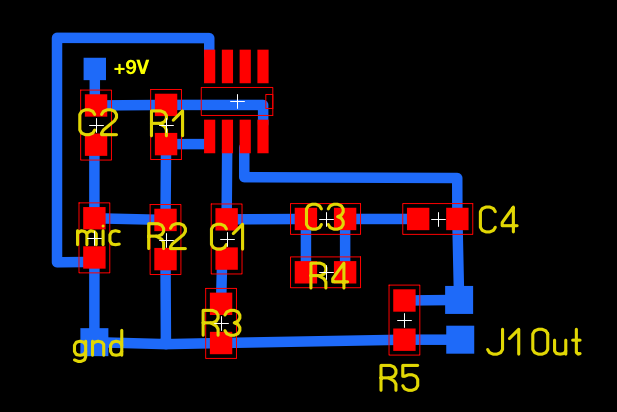
\includegraphics[width=14cm]{sprint-layout-circuit.png}
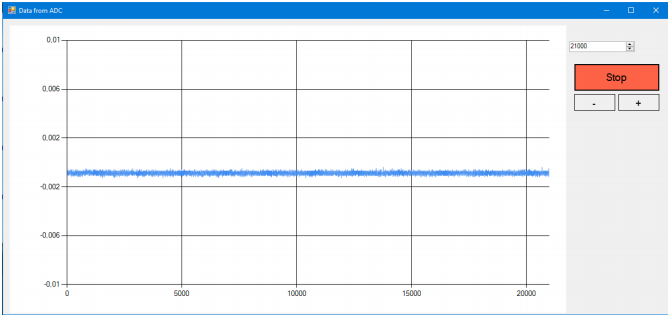
\includegraphics[width=\textwidth]{screenshot.png}
\caption{Скриншот работы программы}
\end{figure}
В центре находится график сигнала с АЦП. Справа находится кнопка старт/стоп, которая управлет запуском и остановкой сбора сигнала с АЦП. Справа вверху есть числовое поле, которое отвечает за количество точек по горизонтальной оси на графике. Кнопки "+/-" Отвечают за увеличение и уменьшение размеров графика (zoom).

\subsection{Описание кода программы}
В начале программы задаются параметры размера буффера и частоты дискретизации (\verb|RATE|).
\begin{verbatim}
const uint   BSIZE              = 524288; // размер буффера
const double RATE               = 8.0e+7;
\end{verbatim}

Далее при нажатии пользователем на кнопку старт, программа начинает инициализацию АЦП. Она проверяет подключено ли устройство, проверяет его работоспособность и начинает сбор данных.

За инициализацию отвечают следующие строчки в коде:
\begin{verbatim}
//========================== ИНИЦИАЛИЗАЦИЯ ================        
st = device.EstablishDriverConnection(BOARD_NAME); //загрузка и 
подключение к библиотеке абстракции устройства
if (st != RSH_API.SUCCESS) SayGoodBye(st);
st  = device.Connect(1); //Подключаемся к устройству. Нумерация с 1.
if (st != RSH_API.SUCCESS) SayGoodBye(st);
p.startType           = (uint)RshInitMemory.StartTypeBit.Program; 
//Запуск сбора данных программный. 
p.bufferSize          = BSIZE; //Размер внутреннего блока данных, 
по готовности которого произойдёт прерывание.
p.frequency           = RATE;  //Частота дискретизации.
p.channels[0].control = (uint)RshChannel.ControlBit.Used;  //Сделаем 0-ой канал активным.
p.channels[0].gain    = 10; // коэффициент усиления для 0-го канала. 
[1, 2, 5, 10] ~ [+-0.2V, +- 0.4V, +-1V, +- 2V]
st = device.Init(p); //Инициализация устройства (передача 
выбранных параметров сбора данных)
if (st != RSH_API.SUCCESS) SayGoodBye(st); //После инициализации 
неправильные значения в структуре будут откорректированы.
\end{verbatim}

Далее программа ждет пока пользователь нажмет кнопку старт. При нажатии на кнопку старт вызывается функция \verb|button1_Click|, которая в свою очередь запускает новый процесс \verb|backgroundWorker1_DoWork|. Этот процесс собирает данные с АЦП в бесконечном цикле пока пользователь не нажмет на кнопку стоп. Он записывает значения с АЦП в структуру данных очередь, доступ к которой имеет UI-процесс (процесс, отвечающий за отображение и обработку элементов пользовательского интерфейса). По мере обновления данных UI процесс обновляет график.

За старт, сбор данных и остановку АЦП отвечает следующий блок кода: 

\begin{verbatim}
double[] buffer = new double[p.bufferSize]; //Получаемый из платы буфер.
uint waitTime = 100000; // Время ожидания(в миллисекундах) до наступления прерывания. Прерывание произойдет при полном заполнении буфера.  // default = 100000
while (getting_data)
{
    stopwatch.Restart();

    st = device.Start(); // Запускаем плату на сбор буфера. по идее нужно для каждого буффера start-stop (в цикле for) Но вроде и так работает и так быстрее намного. (Типа старт за циклом, стоп - внутри for; оба за циклом - не работуют)
    if (st != RSH_API.SUCCESS) SayGoodBye(st);

    st = device.Get(RSH_GET.WAIT_BUFFER_READY_EVENT, ref waitTime);
    if (st != RSH_API.SUCCESS) SayGoodBye(st);

    st = device.GetData(buffer); // very big amount of data
    if (st != RSH_API.SUCCESS) SayGoodBye(st);

    device.Stop();

    // Queue Dequeue and Enqueue implementation with arrays
    double[] values_to_draw_copy = (double[])values_to_draw.Clone();
    for (int i = 0; i < x_axis_points - r_buffer_size; i++) 
        values_to_draw[i] = values_to_draw_copy[r_buffer_size + i];

    for (int i = 0; i < r_buffer_size; i++)
        values_to_draw[x_axis_points - r_buffer_size + i] = buffer[BSIZE / r_buffer_size * i];

    stopwatch.Stop();
    Console.WriteLine("GetData() time:\t" + stopwatch.ElapsedMilliseconds + "ms");
} 
\end{verbatim}

Также процесс backgroundWorker замеряет время каждого цикла сбора данных. (stopwatch.Restart() и stopwatch.Stop()) Это время процесс пользовательского интерфейса выводит на экран.

\subsection{Измерение времени работы АЦП}
Как уже было сказано выше, в зависимости от различных значений размера буффера и частоты дискретизации у АЦП уходит различное время на перезапуск и сбор данных. Эти вычисления производились при помощи стандартной функции-секундомера из стандартной библиотеки C\#.

\subsection{Паралельные вычисления в программе}
В программе используются паралельные вычисления. Присутсвуют два потока. Один поток работает с АЦП: принимает данные и записывает во временный буфер. Другой поток - отрисовывает данные из буффера на графике а также обрабатывает команды пользователя. 

Паралельные вычисления используются из-за необходимости непрерывно получать данные с АЦП, чтобы избежать потери данных. Также, если не использовать паралельные вычисления, то приложение может не реагировать на команды пользователя из за того что процессор будет занят работой с АЦП.

\newpage
\section{Заключение}
В процессе данной работы был создан рабочий прототип устройства, позволяющего анализировать в реальном времени звуковой сигнал, поступающий от сердца или легких. Данное устройство может применяться для получения дополнительной информации, которую человек не может услышать на обычном стетоскопе.

Сфера применения не ограничена медициной, устройство позволяет анализировать любые типы ультразвуковых сигналов.

Развитие проекта можно продолжить в направлении улучшения качества звука. Для этого нужно использовать более дорогие микрофон и усилитель. Также нужно произвести опрос врачей о том, какие именно характеристики звука со стетоскопа важны.

Улучшений в програмном обеспечении можно достигнуть путем оптимизации алгоритмов распаралеливания на нескольких ядрах процессора или на видеокарте. На основе информации от докторов, можно сделать систему распознавания различных забовалеваний легких и сердца.

Разработка данного проекта велась с помощью системы контроля версий git. Исходный код програмного обеспечения, этапы создания и документация доступны по адресу:

\url{https://github.com/tandav/ultrasonic-stethoscope}

\newpage
\renewcommand\refname{Ссылки на источники}
\begin{thebibliography}{}
\bibitem{latexcompanion} 
Аналого цифровой преобразователь ЛА-н10-12USB\\
\url{http://www.rudshel.ru/show.php?dev=14}

\bibitem{latexcompanion} 
Драйверы и програмное обеспечение для устройств ЗАО "Руднев-Шиляев"\\
\url{http://rudshel.ru/software.html}

\bibitem{latexcompanion} 
Документация по программированию устройств ЗАО "Руднев-Шиляев"\\
\url{http://www.rudshel.ru/soft/SDK2/Doc/CPP_USER_RU/html/index.html}

\bibitem{latexcompanion} 
Руководство пользователя ЛА-н10-12USB\\
\url{http://www.rudshel.ru/pdf/LA-n10-12USB(y).rar}

\bibitem{latexcompanion} 
Внешний USB АЦП/ЦАП E14-140-M\\
\url{http://www.lcard.ru/products/external/e-140m)}

\bibitem{latexcompanion} 
Схема усилителя для микрофона\\
\url{http://full-chip.net/analogovaya-elektronika/70-usilitel-dlya-elektretnogo-mikrofona-s-nizkim-urovnem-shuma-shema.html}

\bibitem{latexcompanion} 
Руководство пользователя и технические характеристики операционного усилителя MCP6022\\
\url{https://lib.chipdip.ru/291/DOC000291231.pdf}

\bibitem{latexcompanion} 
Исходный код, документация и этапы создания проекта ультразвукового стетоскопа\\
\url{https://github.com/tandav/ultrasonic-stethoscope}

\end{thebibliography}


\end{document}
